\documentclass[letterpaper]{scrartcl}

\usepackage{tikz,pgfplots}

\begin{document}

\centering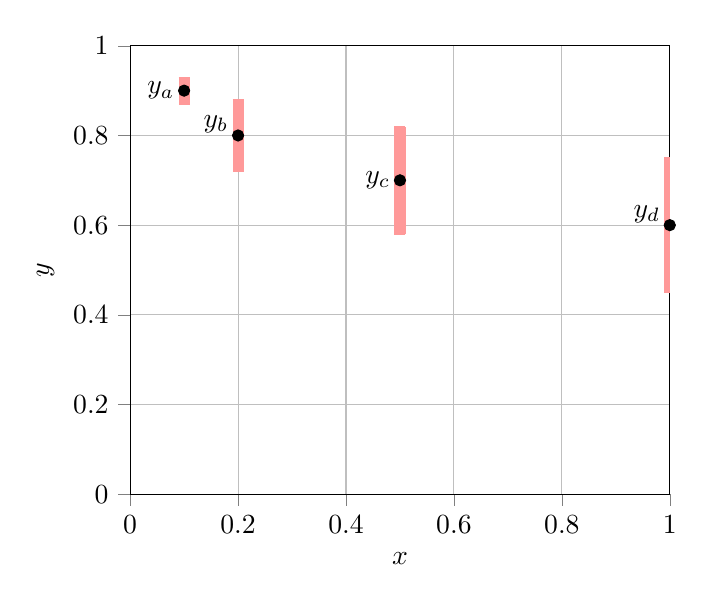
\begin{tikzpicture}[domain=0:1, scale=1]
\begin{axis}[ymin=0, ymax=1, xmin=0, xmax=1,
  ytick={0,0.2,...,1}, ytick align=outside, ytick pos=left,
  xtick={0,0.2,...,1}, xtick align=outside, xtick pos=left,
  xlabel={$x$},
  ylabel={$y$},
  grid=major]
\addplot+[
  only marks,
  mark options={black, scale=1},
  visualization depends on=\thisrow{alignment} \as \alignment,
  nodes near coords,
  point meta=explicit symbolic,
  every node near coord/.style={anchor=\alignment},
  error bars/.cd, 
    y fixed,
    y dir=both, 
    y explicit,
    error bar style={width=4pt, line width=4pt, white!60!red}
] table [x=x, y=y,y error=error, col sep=comma, row sep=crcr, meta index=4] {
    name,  x,      y,  error, label, alignment\\
    a,   0.1,    0.9,   0.03, $y_a$,      0  \\
    b,   0.2,    0.8,   0.08, $y_b$,     -27 \\
    c,   0.5,    0.7,   0.12, $y_c$,      0  \\
    d,   1.0,    0.6,   0.15, $y_d$,     -25 \\
};
\end{axis}
\end{tikzpicture}

\end{document}
